%Chapter 2
\chapter*{Exemplos de elementos formatados}
\addcontentsline{toc}{chapter}{Exemplos de de elementos formatados}
\fancyhead[RO]{\slshape Exemplos de de elementos formatados}  % Mark on right odd pages
\fancyhead[LE]{\slshape Deutschkurs}     % Mark on left even pages

\section*{Equa\c{c}\~ao matemática:}

The Pythagorean theorem states that $a^2 + b^2 = c^2$. We can use the dollar sign also to write isolated math symbols like $\mu$m.

But with double dollar signs we have non-numbered equation, while equation enviroment, we have numbered and referenced equation:
$$ \alpha = \beta^2 + 1 $$
\begin{equation}
  \label{eq:einstein}
  E = mc^2
\end{equation}

In equation \eqref{eq:einstein}, we see the equivalence between mass and energy.

\section*{Figura pós-formata\c{c}\~ao:}
Método H for\c{c}a a figura a ficar exatamente no local onde está colocada no código Latex.
\begin{figure}[H]
    \centering
    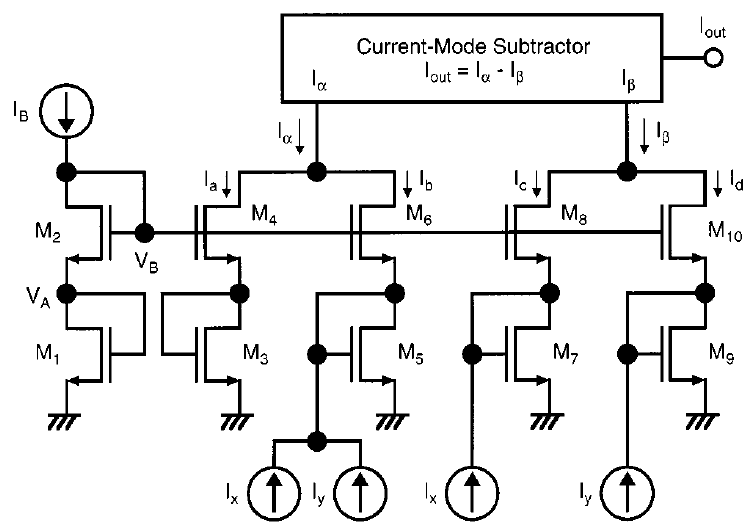
\includegraphics[width=0.8\textwidth]{figures/tanno_multiplier.png}
    \caption{\small Multiplicador de quatro quadrantes proposto em \cite{nunes2023}.\normalsize}
    \label{fig_tanno}
\end{figure}

\section*{Tabela simples:}
Método H for\c{c}a a tabela a ficar exatamente no local onde está colocada no código Latex.
\begin{table}[H]
    \centering
    \caption{Razões de aspecto}
    \label{tab_aspectos}
    \begin{tabular}{|l|r|r|}
    \hline
    Transistor                    & W/L ($\mu$m/$\mu$m) \\ \hline
    M$_1$ e M$_2$                 & 10/0,5              \\ \hline
    M$_3$ a M$_{10}$              & 3,5/0,5             \\ \hline
    M$_{11}$ a M$_{18}$           & 40/0,5              \\ \hline
    M$_{19}$ a M$_{22}$           & 3,5/0,5             \\ \hline
    M$_{1N}$ a M$_{4N}$           & 2,0/0,5             \\ \hline
    M$_{1P}$ a M$_{6P}$           & 20/0,5              \\ \hline
    \end{tabular}
\end{table}
